%@descr: wzór sprawozdania, raportu lub pracy - nadaje się do przeróbek
%@author: Maciej Komosiński

\documentclass{article} 
\usepackage{polski} %moze wymagac dokonfigurowania latexa, ale jest lepszy niż standardowy babel'owy [polish] 
\usepackage[utf8]{inputenc} 
\usepackage[OT4]{fontenc} 
%\usepackage{gensymb}
\usepackage{graphicx,color} %include pdf's (and png's for raster graphics... avoid raster graphics!) 
\usepackage{url} 
\usepackage[pdftex,hyperfootnotes=false,pdfborder={0 0 0},colorlinks=true, linkcolor=blue]{hyperref} %za wszystkimi pakietami; pdfborder nie wszedzie tak samo zaimplementowane bo specyfikacja nieprecyzyjna; pod miktex'em po prostu nie widac wtedy ramek


% Zmiana rozmiarów strony tekstu
\addtolength{\voffset}{-1cm}
\addtolength{\hoffset}{-1cm}
\addtolength{\textwidth}{2cm}
\addtolength{\textheight}{2cm}

%bardziej zyciowe parametry sterujace rozmieszczeniem rysunkow
\renewcommand{\topfraction}{.85}
\renewcommand{\bottomfraction}{.7}
\renewcommand{\textfraction}{.15}
\renewcommand{\floatpagefraction}{.66}
\renewcommand{\dbltopfraction}{.66}
\renewcommand{\dblfloatpagefraction}{.66}
\setcounter{topnumber}{9}
\setcounter{bottomnumber}{9}
\setcounter{totalnumber}{20}
\setcounter{dbltopnumber}{9}

% własny bullet list z malymi odstepami
\newenvironment{tightlist}{
\begin{itemize}
  \setlength{\itemsep}{1pt}
  \setlength{\parskip}{0pt}
  \setlength{\parsep}{0pt}}
{\end{itemize}}

%obrazkow szukamy w nastepujacym katalogu:
\graphicspath{{pics/}}



%\title{Sprawozdanie z laboratorium:\\Metaheurystyki i Obliczenia Inspirowane Biologicznie}
%\author{}
%\date{}


\begin{document}

\thispagestyle{empty} %bez numeru strony

\begin{center}
{\large{Sprawozdanie z laboratorium:\\
Informatyka w Medycynie\\
(szablon)}}

\vspace{3ex}

Część I: Symulator tomografu komputerowego
%Część II: Algorytmy optymalizacji lokalnej i globalnej, problem QAP
%Część III: Eksperyment: ... (prezentację można zrobić w LaTeX - służy do tego klasa "beamer")

\vspace{3ex}
{\footnotesize\today}

\end{center}


\vspace{10ex}

Prowadzący: mrg inż. Iwo Błądek

\vspace{5ex}

Autorzy:
\begin{tabular}{lllr}
\textbf{Sebastian Firlik} & inf122485 & I2 & sebastian.firlik@student.put.poznan.pl \\
\textbf{Piotr Hankiewicz} & inf1225** & I2 & MAIL \\
\end{tabular}

\vspace{5ex}

Zajęcia piątkowe, 11:45.

\vspace{35ex}

\noindent Oświadczam/y, że niniejsze sprawozdanie zostało przygotowane wyłącznie przez powyższych autora/ów,
a wszystkie elementy pochodzące z innych źródeł zostały odpowiednio zaznaczone i~są cytowane w bibliografii.  

\newpage



\section*{Udział autorów}
\begin{tightlist}
\item SF zaimplementował tworzenie sinogramu, a także jego zapis do formatu DICOM, przygotował środowisko graficzne aplikacji
\item PH zaimplementował odtwarzanie obrazu wejściowego na podstawie sinogramu wraz z filtrowaniem, przeprowadził eksperyment wyjaśniający wpływ niżej opisanych parametrów na jakoś odtwarzanego obrazu.
\end{tightlist}



\section{Wstęp}

Naszym zadaniem było stworzenie aplikacji desktopowej w wybranej technologii i zaimplementowanie w niej symulacji dwuwymiarowego tomografu komputerowego. Wszystkie wymagania zostały wypunktowane \href{https://www.cs.put.poznan.pl/ibladek/students/iwm/0_projekt_wspolny_Tomograf.pdf}{tutaj}. Do stworzenia naszej aplikacji użyliśmy:
\begin{tightlist}
\item języka Python 3,
\item środowiska PyQt5 do stworzenia interfejsu okienkowego,
\item bibliotek dostępnych w języku Python (matplotlib, numpy, pyDicom...)
\end{tightlist}

Jedynie do obsługi zapisu do formatu DICOM użyliśmy gotowej biblioteki ze względu na trudność manipulacji danymi w tym formacie. Wszystkie obliczenia, zarówno podczas generacji sinogramu, jak i przejściu do obrazu wynikowego, a także obrót emitera i detektorów w funkcji kąta zamodelowaliśmy samodzielnie.

\subsection{Dyskretna Transformata Radona}
\begin{figure}[!htbp]
\begin{center}
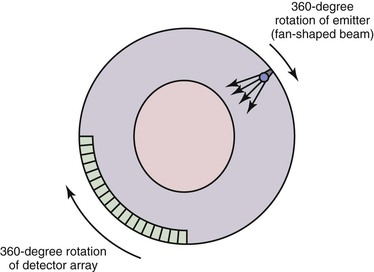
\includegraphics[width=0.8\textwidth]{tomograf.jpg}
\end{center}
\caption{Schemat działania tomografu}
\label{fig:1Tdelta}
\end{figure}

Na Rysunku 1 widzimy, jak działa nasz tomograf komputerowy - jeden emiter obraca się o $360 ^{\circ}$, wysyła promieniowanie rentgenowskie przez badany obiekt i każda wiązka trafia na odpowiedni detektor. W naszej symulacji, przy pomocy algorytmu Bresenhama tworzymy dyskretną linię, prowadzącą od emitera do detektora przez obraz i sumuje jasności pikseli na tej drodze. W ten sposób, na każdej ścieżce emiter-detektor, dla każdego możliwego kąta obrotu emitera, otrzymujemy \textbf{sinogram}, czyli pośredni etap wizualizacji badanego obiektu. Nie podlega on żadnej analizie diagnostycznej. Następnie w wyniku operacji odwrotnej (Odwrotna Dyskretna Transformata Radona) otrzymujemy obraz wynikowy. 

\subsection{Odwrotna Dyskretna Transformata Radona
}
ODTR polega na tym, że z każdym kątem obrotu $\alpha$ i każdą parą emiter-detektor sprzężona jest suma jasności pikseli na ich drodze. Na każdym pikselu, znajdującym się na tej drodze, zostawiamy średnią jasność odpowiedniego piksela, wynikającą z sumy z sinogramu. Po iteracyjnym odtworzeniu obrazu, bez nałożonego filtrowania widzimy niedokładny, rozmyty obraz, podobny do początkowego. 

\subsection{Normalizacja}

Po wygenerowaniu wynikowego obrazka, należało dane znormalizować. 

\begin{equation}
obrazek = \frac{obrazek - min(obrazek)}{max(obrazek)-min(obrazek)} * 255
\end{equation}

Od każdego piksela naszego obrazka odejmujemy minimalną jasność z całego wynikowego obrazu i dzielimy to przez różnicę między najjasniejszym i najciemniejszym pikselem. Następnie mnożymy każdy piksel obrazka przez 255, by otrzymać wartości z przedziału [0, 255]. Dzięki temu upewniamy się, że najciemniejsze punkty wygenerowanego obrazu będą czarne (a nie szare, jak wynikałoby z działania Odwrotnej Transformaty Radona -- rozkłada jasność równomiernie na całej linii, więc praktycznie żadne piksele nie mogłyby być czarne i różnica między wygenerowany obrazem a obrazem pierwotnym byłaby kolosalna) a najjaśniejsze białe.

Na poniższych rysunkach widzimy jak wygląda krok pośredni generowania obrazu (sinogram -- Rysunek 3) a także obraz końcowy (Rysunek 4).

\begin{figure}[!htbp]
\begin{center}
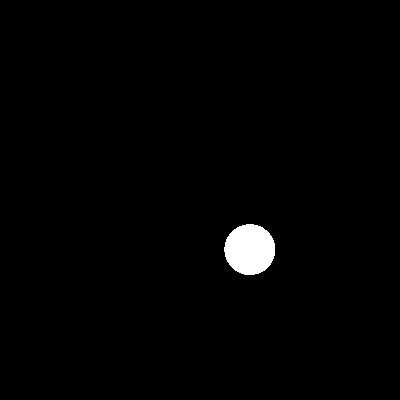
\includegraphics[width=0.4\textwidth]{Kropka.jpg}
\end{center}
\caption{Obraz początkowy}
\label{fig:1Tdelta}
\end{figure}

\begin{figure}[!htbp]
\begin{center}
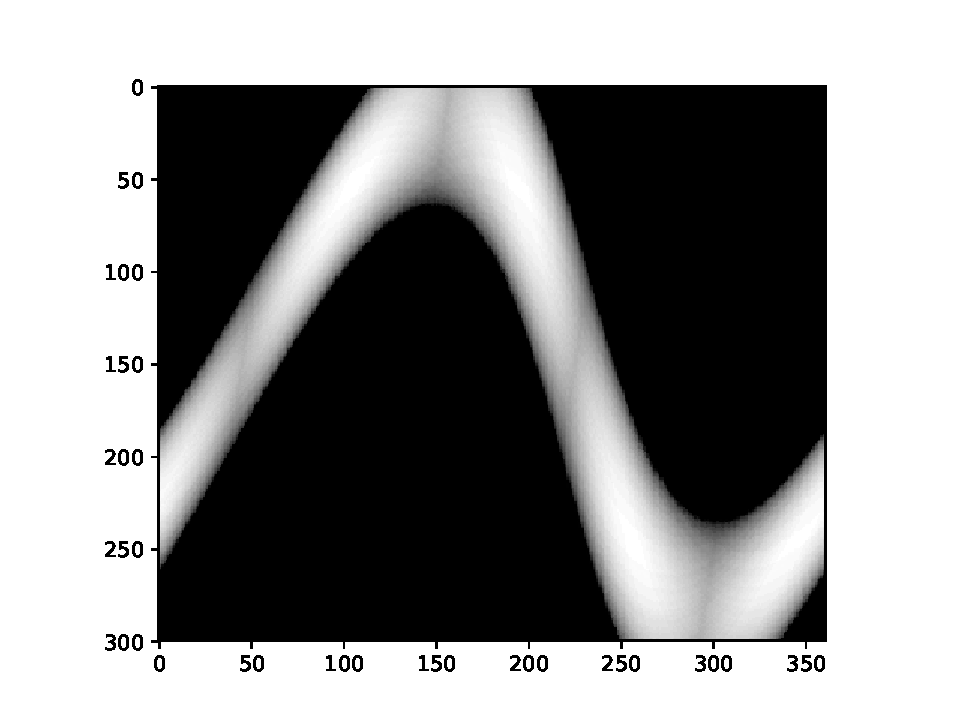
\includegraphics[width=0.8\textwidth]{foo.pdf}
\end{center}
\caption{Wygenerowany sinogram}
\label{fig:1Tdelta}
\end{figure}

\begin{figure}[!htbp]
\begin{center}
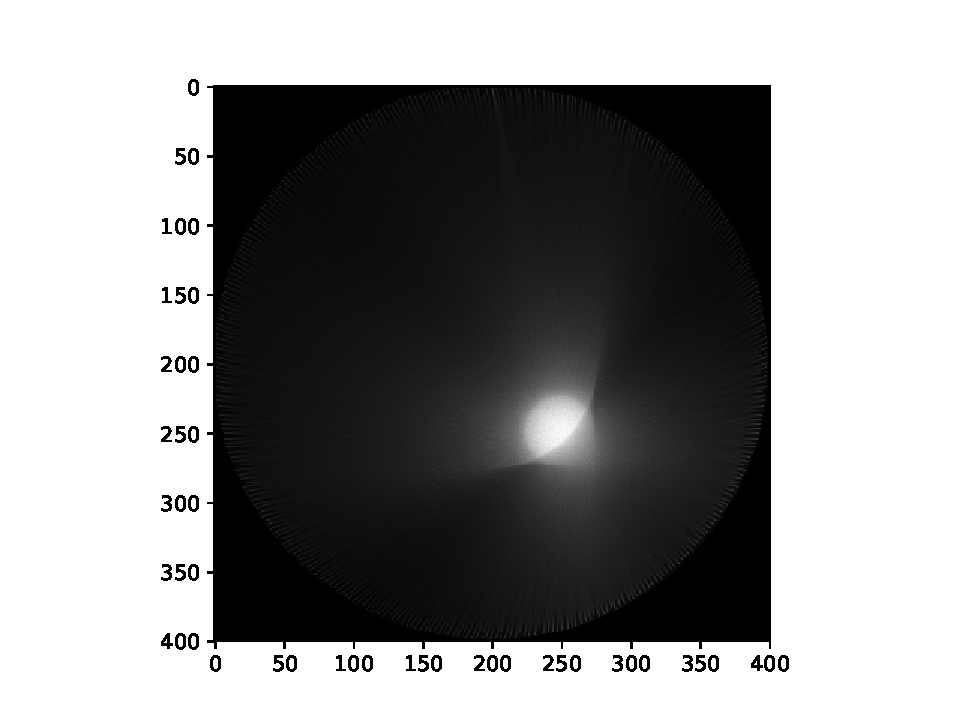
\includegraphics[width=0.8\textwidth]{result.pdf}
\end{center}
\caption{Obraz wynikowy}
\label{fig:1Tdelta}
\end{figure}

\clearpage %pozwol umiescic zalegle rysunki od razu tutaj 


\section{Analiza statystyczna}
\label{sec_analiza_statystyczna}

\subsection{Wpływ kąta $\alpha$ na jakość przetwarzania}
\label{subsec_alpha_comparison}

Pierwszym z parametrów wpływających na jakość przetwarzania jest kąt o jaki obraca się emiter w jednej iteracji. 

%\begin{figure}[!htbp]
%\begin{center}
%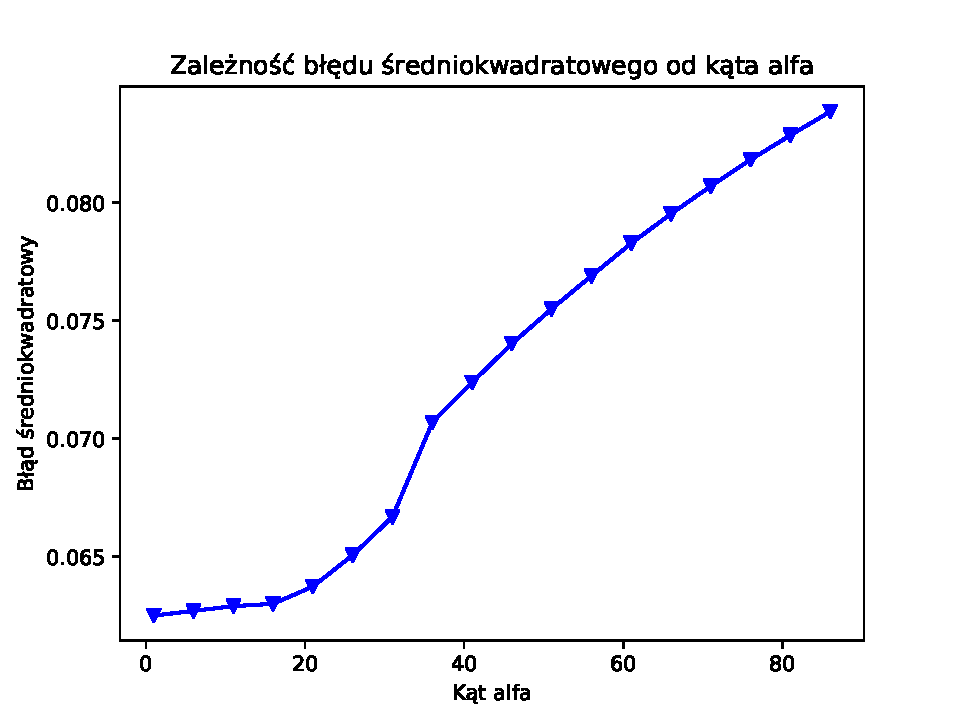
\includegraphics[width=0.8\textwidth]{alpha.pdf}
%\end{center}
%\caption{Wpływ kąta alfa na jakość przetwarzania}
%\label{fig:detectors_amount}
%\end{figure}

Jak widać na poniższym wykresie wraz ze wzrostem wartości kąta alfa wzrasta też wartość błędu średniokwadratowego. Wynika to z faktu, że im większy omawiany kąt tym mniej razy nastąpi zebranie informacji o obiekcie, a co za tym idzie obraz wyjściowy będzie coraz mniej dokładny. 
Przeprowadzona analiza wskazuje, że początkowo wartość błędu zwiększa się w nieznacznym stopniu, by dla wartości w przedziale $\left[ 35; 40 \right]$ osiągnąć największy skok wartości. Następnie, aż do końca eksperymentu błąd rośnie liniowo względem zmiany wartości kąta alfa.

\subsection{Wpływ liczby detektorów na jakość przetwarzania}
\label{subsec_detectors_amount_comparison}



Kolejnym z czynników jest liczba detektorów. Na osi y przedstawione są wartości błędu średniokwadratowego dla kolejnych wartości liczb detektorów, które znajdują się na osi x. 

%\begin{figure}[!htbp]
%\begin{center}
%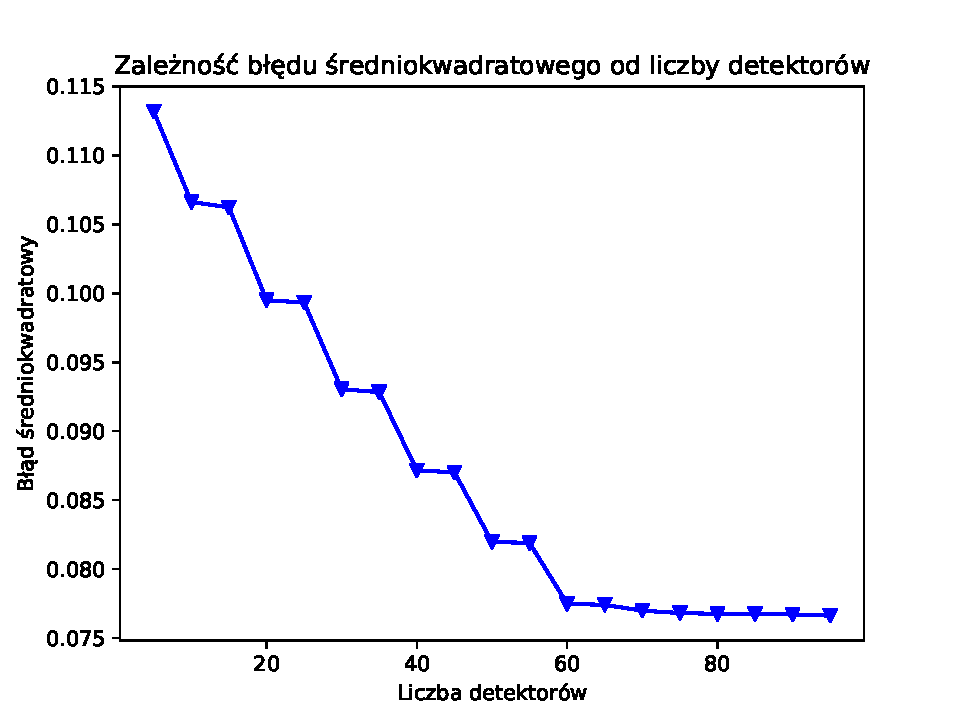
\includegraphics[width=0.8\textwidth]{detectors_amount.pdf}
%\end{center}
%\caption{Wpływ liczby detektorów na jakość przetwarzania}
%\label{fig:detectors_amount}
%\end{figure}

Wraz ze zwiększeniem liczby detektorów spada błąd średniokwadratowy. Wynika to z faktu, że im więcej detektorów w modelu tomografu tym gęściej wysyłane są wiązki z danego emitera, co skutkuje dokładniejszym obrazem. Spowodowane jest to tym, że im więcej wiązek jest wysyłanych tym mniej niezarejestrowanych przez nie pikseli. W takich sytuacjach, piksele, przez które nie przechodziła wiązka, na obrazie wyjściowym będą miały kolor czarny.

Należy zaznaczyć, że po przekroczeniu granicznej liczby detektorów, która zależna jest od pozostałych parametrów przetwarzania zmiana błędu średniokwadratowego stabilizuje się, zmienia się w bardzo niewielkim stopniu, pomimo początkowego bardzo wyraźnego spadku.
W naszym eksperymencie, pozostałe parametry czyli kąt alfa i rozpiętość kątowa została ustalona na wartości odpowiednio $5 ^{\circ}$ i $180 ^{\circ}$. Dla tak przyjetych parametrów omawiana wartość graniczna ustalila się na wartość 60. 

\subsection{Wpływ rozpiętości kątowej detektorów na jakość przetwarzania}
\label{subsec_cone_width_comparison}

Ostatnim z czynników wpływających na przetwarzanie jest rozpiętość kątowa detektorów. Na osi y przedstawione są wartości błędu średniokwadratowego dla kolejnych wartości liczby detektorów, które znajdują się na osi x.

%\begin{figure}[!htbp]
%\begin{center}
%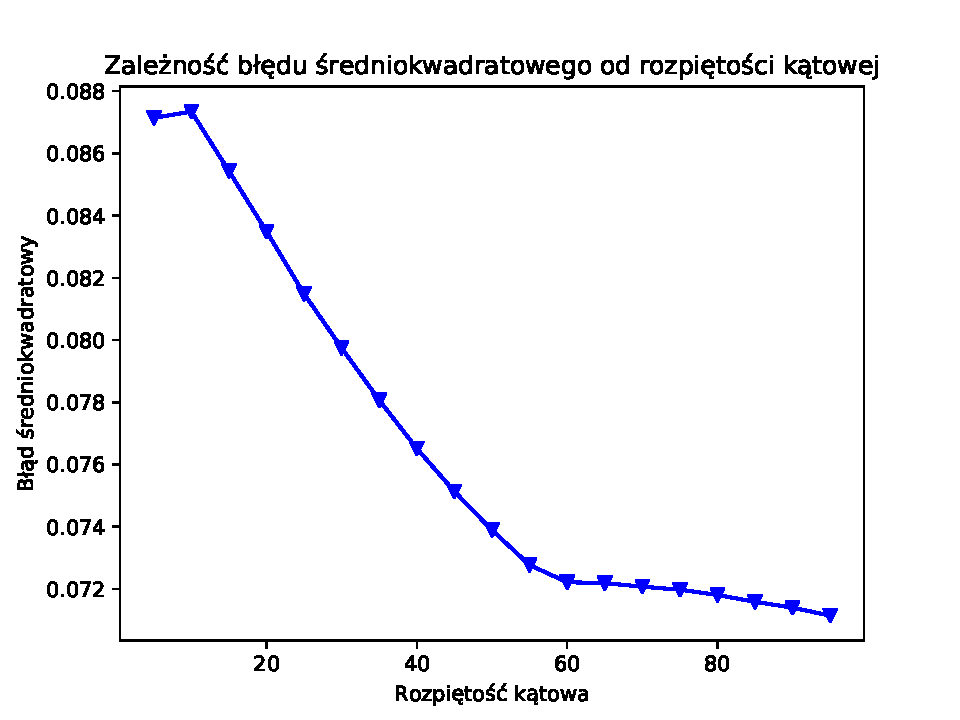
\includegraphics[width=0.8\textwidth]{cone_width.pdf}
%\end{center}
%\caption{Wpływ rozpiętości kątowej na jakość przetwarzania}
%\label{fig:cone_width}
%\end{figure}

Wraz ze zwiększeniem rozpiętości kątowej detektorów spada błąd średniokwadratowy. Wynika to z  faktu, że im szersze spektrum widzenia tym mniej elementów jest nieobjętych wiązkami w danej iteracji. Pełny obrót tomografu zapewnia zebranie informacji o obiekcie, jednakże im szerszy "kąt widzenia" tomografu, tym więcej zebranych o nim danych.

W początkowej fazie eksperymentu zaobserwować można gwałtowny spadek błędu średniokwadratowego. W odróżnieniu od poprzedniego przypadku, nie ma nagłej zmiany tendencji. Spadek wartości błędu średniokwadratowego zaczyna być powolniejszy, by osiągnąć względną stabilizację. Po osiągnięciu wartości $60^{\circ}$ obserwuje się niewielki spadek wartości aż do końca eksperymentu.

\section{Filtr}

%%%%%%%%%%%%%%%% literatura %%%%%%%%%%%%%%%%

\bibliography{sprawozd}
\bibliographystyle{plain}


\end{document}

